\documentclass[11pt, a4paper]{article}

\usepackage[margin=1in]{geometry}
\usepackage{graphicx}
\usepackage{amsmath, amssymb}
\usepackage[dvipsnames]{xcolor}
\usepackage{hyperref}
\usepackage{booktabs}
\usepackage{float}
\usepackage[font=small, labelfont=bf]{caption}
\usepackage{parskip}
\usepackage{enumitem}

\hypersetup{
    colorlinks=true,
    linkcolor=blue!60!black,
    citecolor=blue!60!black,
    urlcolor=blue!60!black,
}

\title{\textbf{Learned Index Structures}\\[0.3em]
\large From Foundational Theory to the 2026 State of the Art}
\author{}
\date{}

\begin{document}
\maketitle

\begin{abstract}
Traditional index structures---B-trees, hash maps, binary search---treat data generically,
making no assumptions about the distribution of keys. Learned indexes replace these
branchy, pointer-chasing structures with mathematical models that predict where data lives.
This report explains the core idea, walks through the progression from naive linear models
to piecewise linear approximations, analyzes performance tradeoffs, surveys the state
of the art through 2026---including concurrent indexes, LSM-tree integration, and
auto-tuning---and discusses the gap between research results and production adoption.
\end{abstract}

\tableofcontents
\newpage

%% ====================================================================
\section{The Core Insight}

Every index structure is a function. Given a key $k$, the index returns a position $p$
in a sorted collection where $k$ can be found:

\[
    \text{index}: k \mapsto p
\]

A B-tree implements this function through a series of comparisons, traversing nodes
from root to leaf. Each node comparison is a potential cache miss---fetching a 64-byte
cache line from main memory, waiting ${\sim}100$ nanoseconds, comparing, then chasing
a pointer to the next node. For $N = 10^6$ keys, a B-tree with fanout 16 requires
$\lceil \log_{16}(10^6) \rceil \approx 5$ levels, each potentially a cache miss.

But if your keys follow a known distribution, you don't need a tree. A mathematical
model can predict the position directly.

\subsection{Keys as a Cumulative Distribution Function}

If you sort $N$ keys and plot each key's value against its rank (position), you get
the \textbf{cumulative distribution function} (CDF) of the key distribution. For
uniformly distributed keys, this is a straight line.

\begin{figure}[H]
    \centering
    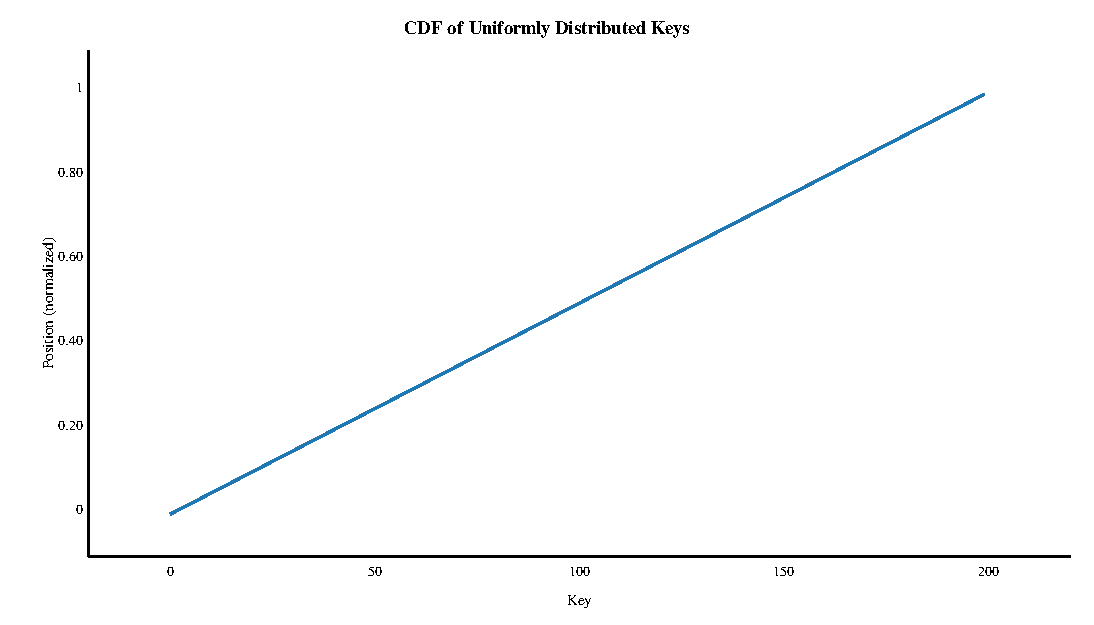
\includegraphics[width=0.85\textwidth]{figures/cdf_uniform.pdf}
    \caption{CDF of uniformly distributed keys. The relationship between key and
    position is perfectly linear---a single multiply and add predicts the exact position.}
    \label{fig:cdf-uniform}
\end{figure}

For real-world data---timestamps clustered around business hours, IP addresses
clustered by subnet---the CDF is nonlinear but still smooth and monotonically increasing.

\begin{figure}[H]
    \centering
    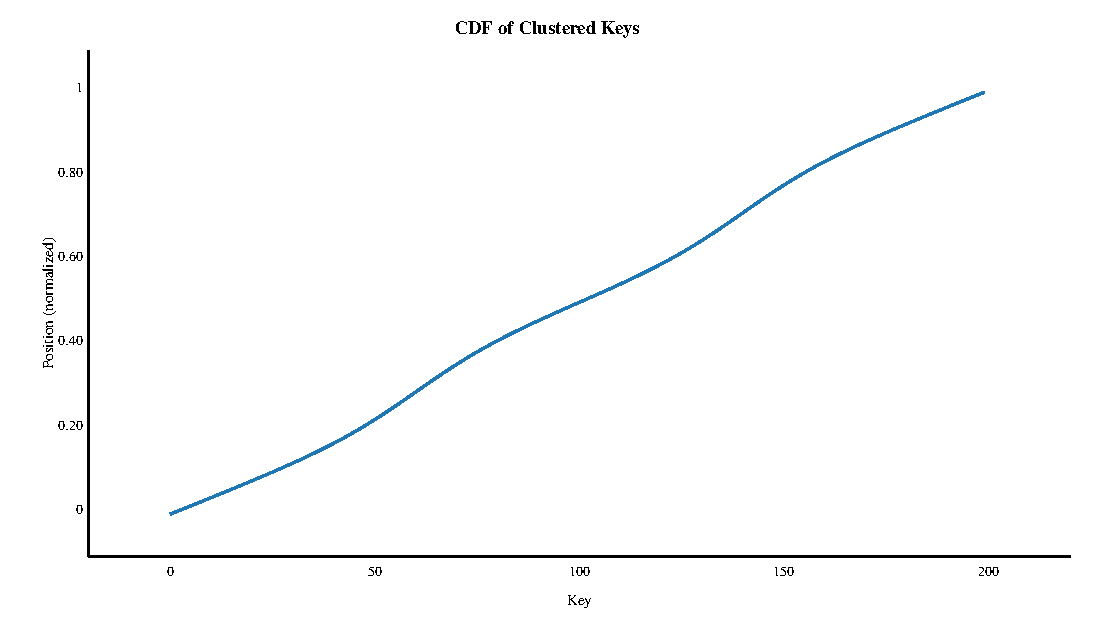
\includegraphics[width=0.85\textwidth]{figures/cdf_clustered.pdf}
    \caption{CDF of clustered keys. The S-curve shape reflects regions of high
    key density (steep slope) and low density (shallow slope).}
    \label{fig:cdf-clustered}
\end{figure}

The key observation from Kraska et al.\ (2018): \emph{an index is just a model of the CDF}.
A B-tree is a general-purpose CDF estimator. A learned index is a specialized one,
fit to the actual data distribution.

%% ====================================================================
\section{From Linear Models to Piecewise Approximation}

\subsection{The Naive Approach: A Single Linear Model}

The simplest learned index fits a single linear function to the CDF:

\[
    \hat{p} = \frac{k - k_{\min}}{k_{\max} - k_{\min}} \cdot N
\]

For uniform keys, this is nearly perfect. For clustered keys, the fit is poor.

\begin{figure}[H]
    \centering
    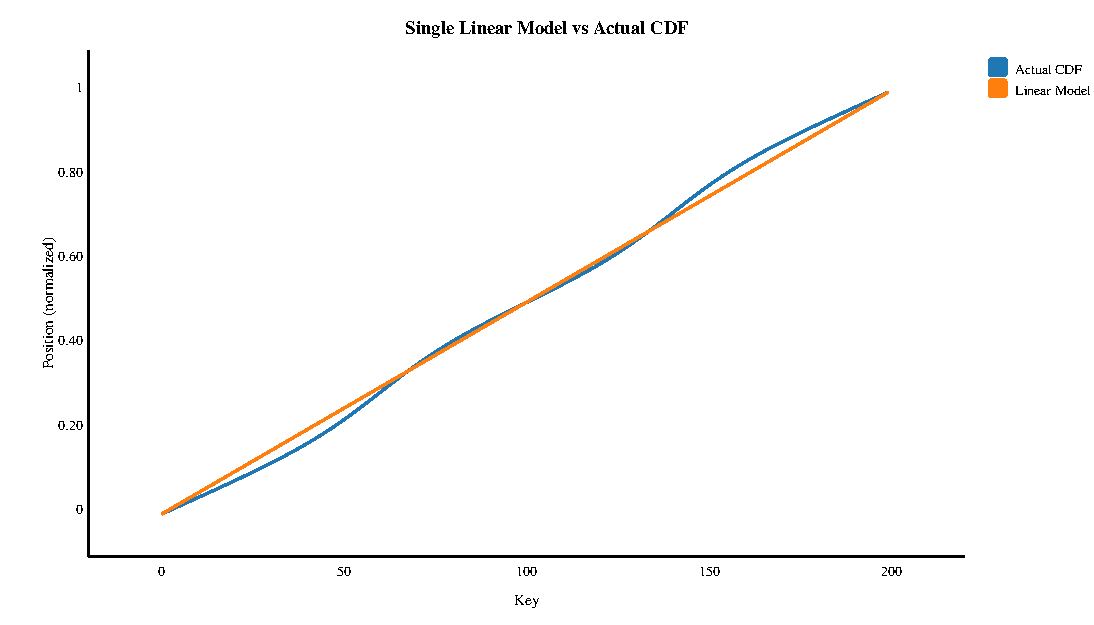
\includegraphics[width=0.85\textwidth]{figures/linear_vs_cdf.pdf}
    \caption{A single linear model overlaid on a clustered CDF. The model
    systematically over-predicts in sparse regions and under-predicts in dense regions.}
    \label{fig:linear-vs-cdf}
\end{figure}

The prediction error can be substantial. In areas where the CDF curves away from
the linear approximation, the model's predicted position can be off by hundreds
of positions, requiring a costly correction scan.

\begin{figure}[H]
    \centering
    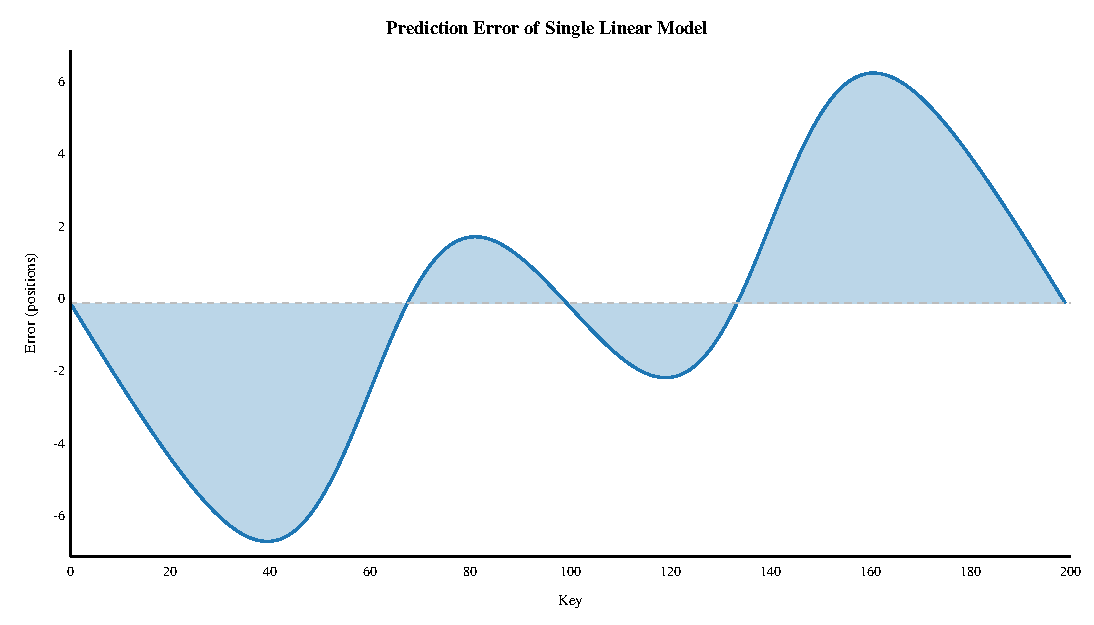
\includegraphics[width=0.85\textwidth]{figures/linear_error.pdf}
    \caption{Prediction error (in number of positions) of a single linear model.
    Errors concentrate at the transitions between dense and sparse key regions.}
    \label{fig:linear-error}
\end{figure}

\subsection{Piecewise Linear Models: The PGM-Index}

The solution is to break the key space into \textbf{segments}, each covered by its
own linear model. Within each segment, the model achieves a guaranteed maximum
error of $\varepsilon$ positions.

Each segment is defined by three values:

\[
    \text{Segment} = (\text{start\_key}, \text{slope}, \text{intercept})
\]

A lookup proceeds as:

\begin{enumerate}[nosep]
    \item Find which segment covers the query key (binary search over segment start keys).
    \item Predict: $\hat{p} = \text{slope} \cdot k + \text{intercept}$.
    \item Scan at most $\varepsilon$ positions in either direction.
\end{enumerate}

The total cost is one binary search over a small number of segments (or a recursive
learned model over the segments themselves), one multiply-add, and a bounded local scan.

\begin{figure}[H]
    \centering
    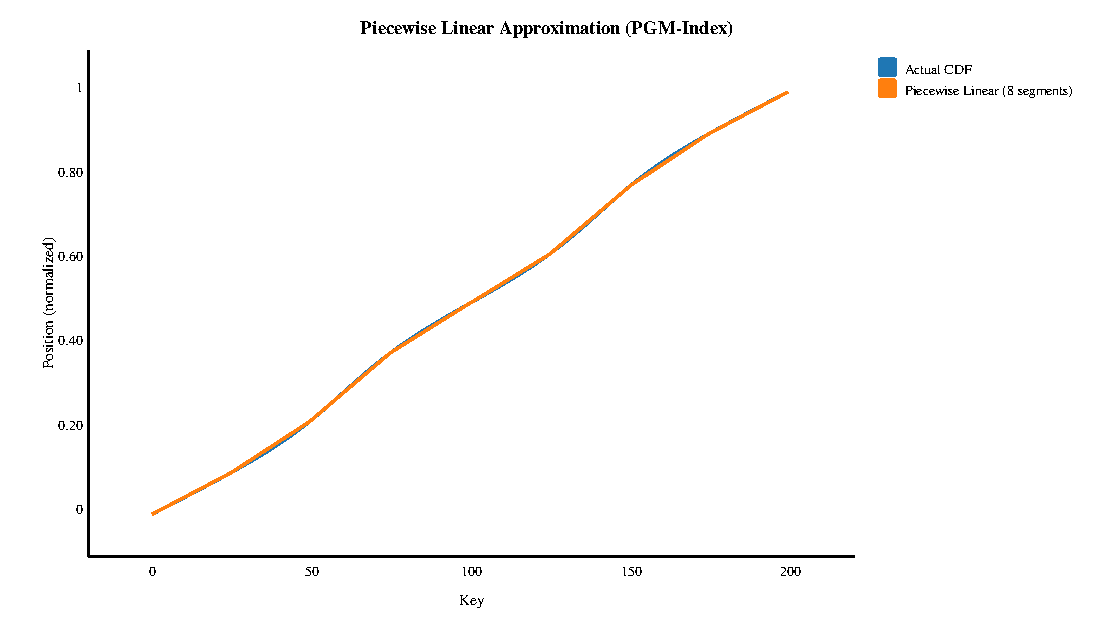
\includegraphics[width=0.85\textwidth]{figures/pgm_fit.pdf}
    \caption{Piecewise linear approximation with 8 segments. The fit tracks the
    CDF far more closely than a single linear model, especially in transition regions.}
    \label{fig:pgm-fit}
\end{figure}

The improvement in prediction accuracy is dramatic:

\begin{figure}[H]
    \centering
    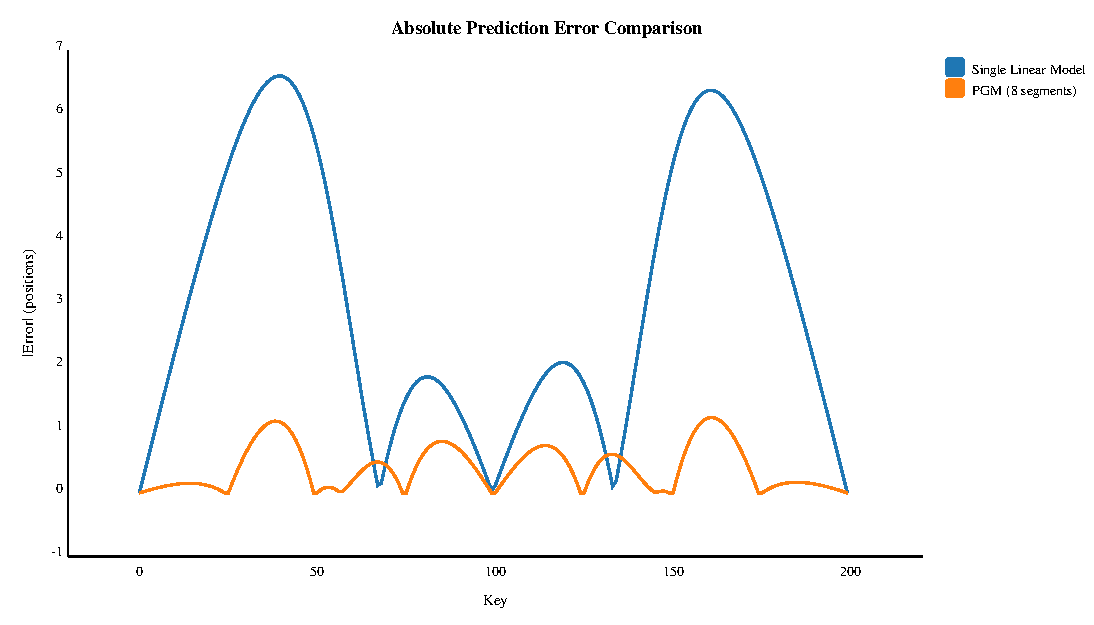
\includegraphics[width=0.85\textwidth]{figures/error_comparison.pdf}
    \caption{Absolute prediction error: single linear model vs.\ piecewise
    linear with 8 segments. The piecewise model reduces maximum error by
    an order of magnitude.}
    \label{fig:error-comparison}
\end{figure}

\subsection{Recursive Structure}

The PGM-Index is elegant because it is \textbf{recursive}. The segments at the
bottom level approximate the data CDF. But the segment start keys themselves
form a sorted array---which can be indexed by another layer of piecewise linear
models. You stack layers until the top level fits in a single model:

\begin{center}
\begin{tabular}{ll}
    \toprule
    \textbf{Level} & \textbf{Role} \\
    \midrule
    Level 0 (top) & 1 model, predicts which Level-1 segment to use \\
    Level 1       & $\sim$10 segments, each predicts into Level-2 \\
    Level 2       & $\sim$1000 segments, each predicts into the data \\
    Data          & Sorted array of key-value pairs \\
    \bottomrule
\end{tabular}
\end{center}

In practice, 2--3 levels suffice for billions of keys. Each level adds one
multiply-add operation (CPU registers, no cache miss) to the lookup path.

\subsection{Where the Bottleneck Actually Is: PGM++ (2025)}

Recent analysis by Liu et al.\ (PVLDB 2025) revealed a surprising finding:
the performance bottleneck in PGM-Index is \textbf{not} the model prediction
itself, but the \textbf{error-bounded search} within segments. This internal
search is memory-bound---the correction scan after prediction dominates
wall-clock time.

Their PGM++ system replaces the error-bounded binary search with a hybrid
search strategy and adds an automatic hyper-parameter tuner, achieving
2.31$\times$ speedup over the original PGM-Index and 1.56$\times$ over
optimized RMI. This suggests that future work on learned indexes should
focus as much on the \emph{last-mile search} as on improving model accuracy.

%% ====================================================================
\section{The $\varepsilon$ Tradeoff}

The error bound $\varepsilon$ is the fundamental tuning parameter. It controls
the tradeoff between model size (number of segments) and correction scan length.

\begin{figure}[H]
    \centering
    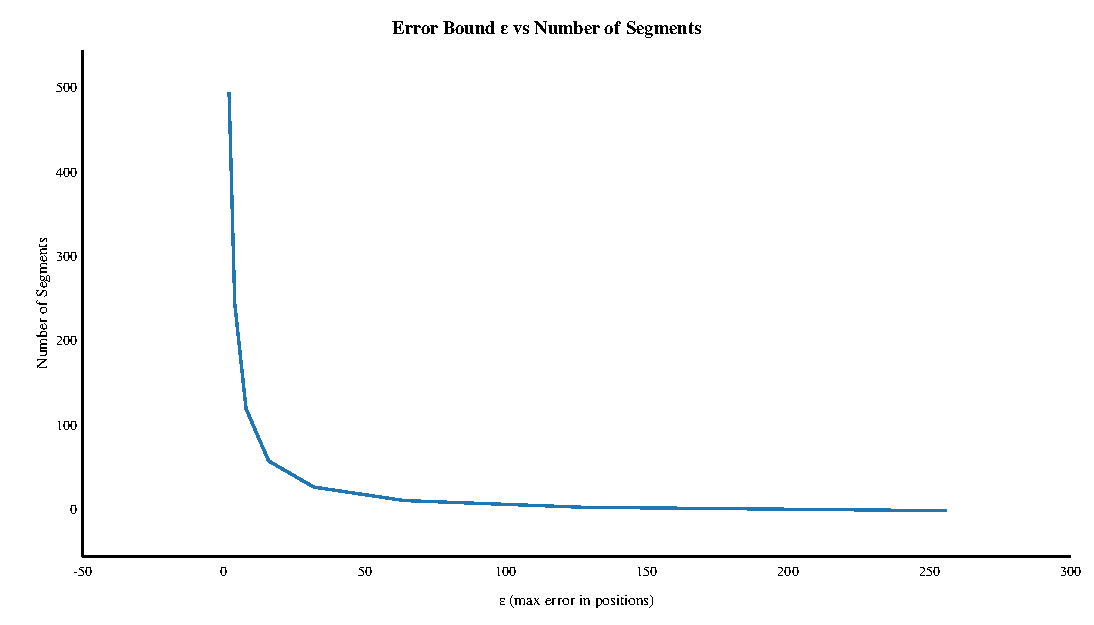
\includegraphics[width=0.85\textwidth]{figures/epsilon_tradeoff.pdf}
    \caption{As the error bound $\varepsilon$ grows, fewer segments are needed
    (less memory), but each lookup may require scanning more positions.}
    \label{fig:epsilon}
\end{figure}

\begin{itemize}[nosep]
    \item \textbf{Small $\varepsilon$}: More segments (higher memory), but
        correction scans are short and cache-friendly.
    \item \textbf{Large $\varepsilon$}: Fewer segments (less memory), but
        correction scans may span multiple cache lines.
\end{itemize}

The optimal $\varepsilon$ depends on the hardware's cache line size and memory
latency. On modern x86 CPUs, $\varepsilon \in [32, 128]$ typically balances
memory overhead against scan cost.

LITune (SIGMOD 2025) takes this further by using \textbf{deep reinforcement
learning} to auto-tune $\varepsilon$ and other parameters end-to-end, achieving
up to 98\% runtime reduction and 17$\times$ throughput increase over default
configurations. This suggests that the ``right'' $\varepsilon$ is not a single
value but a function of the workload, hardware, and data distribution---too
complex for manual tuning.

%% ====================================================================
\section{Why This Beats B-Trees on Modern Hardware}

\subsection{Cache Misses}

B-trees were designed when CPU speed and memory speed were comparable. Today,
a CPU cycle takes ${\sim}0.3$ ns while a main memory access takes ${\sim}100$ ns---a
300$\times$ gap. Every pointer chase in a B-tree is a potential cache miss.

A learned index replaces pointer chasing with arithmetic. The model evaluation
(multiply, add, compare) operates entirely in CPU registers or L1 cache. Only
the final correction scan touches the data array, and it accesses sequential
memory (cache-line friendly).

\begin{figure}[H]
    \centering
    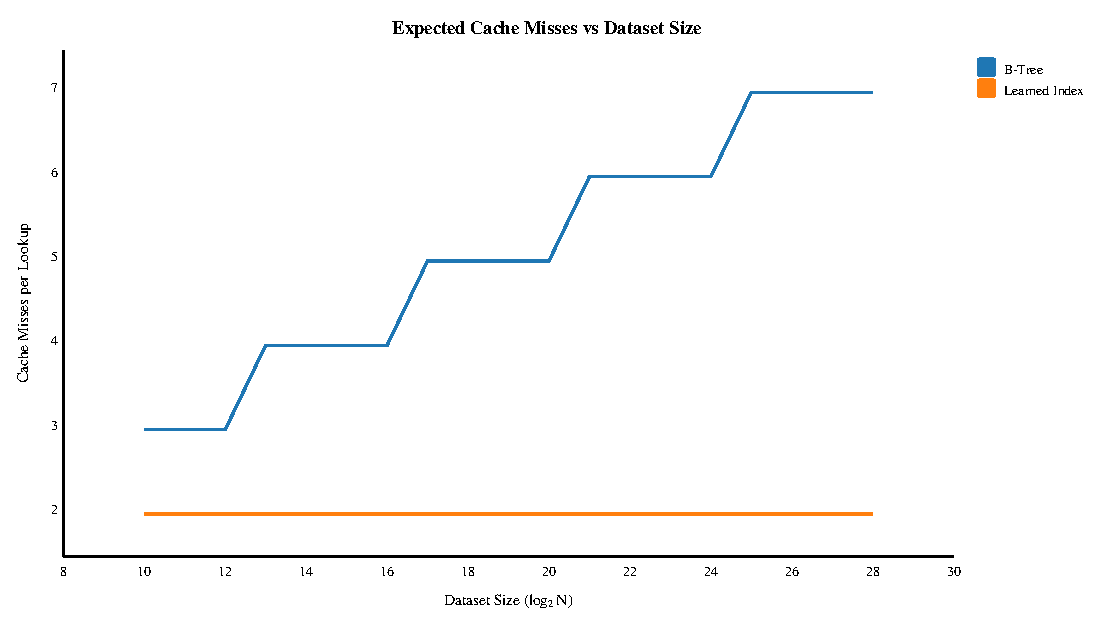
\includegraphics[width=0.85\textwidth]{figures/cache_misses.pdf}
    \caption{Expected cache misses per lookup as dataset size grows. B-tree
    misses grow logarithmically with $N$; learned index misses remain nearly constant.}
    \label{fig:cache-misses}
\end{figure}

\subsection{Lookup Cost}

\begin{figure}[H]
    \centering
    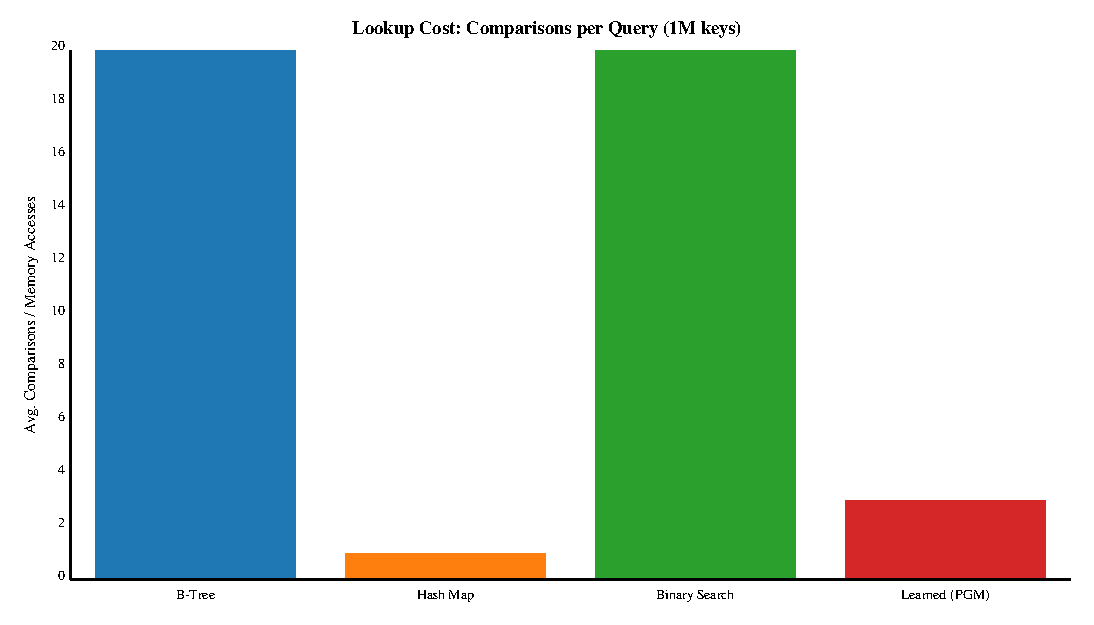
\includegraphics[width=0.85\textwidth]{figures/lookup_cost.pdf}
    \caption{Average comparisons or memory accesses per lookup for 1M 64-bit
    integer keys. Hash maps offer $O(1)$ but sacrifice ordering. Learned
    indexes approach hash map speed while maintaining sorted order.}
    \label{fig:lookup-cost}
\end{figure}

\subsection{Memory Efficiency}

\begin{figure}[H]
    \centering
    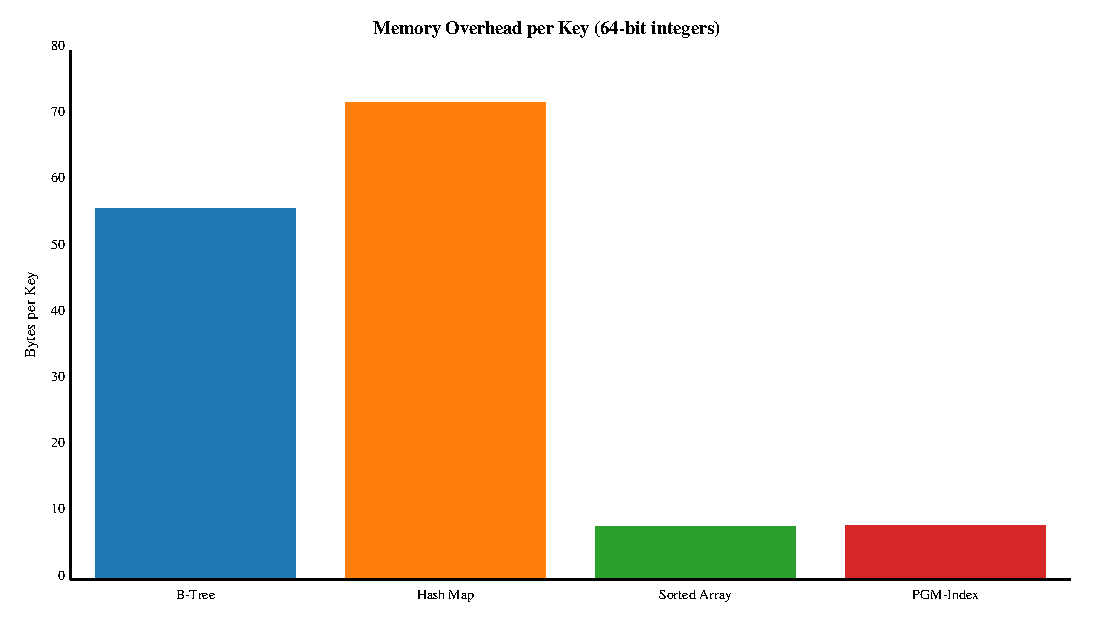
\includegraphics[width=0.85\textwidth]{figures/memory_usage.pdf}
    \caption{Memory overhead per key. B-trees and hash maps carry significant
    per-node/per-bucket overhead. The PGM-Index stores data in a raw sorted array
    with minimal auxiliary structure (a few bytes of model parameters per segment).}
    \label{fig:memory}
\end{figure}

%% ====================================================================
\section{Real-World Key Distributions}

Real datasets are rarely uniform. Timestamps cluster around business hours.
IP addresses cluster by subnet. Database primary keys may be sequential with
gaps from deletions. Learned indexes exploit these patterns---the more
predictable the distribution, the fewer segments are needed and the tighter
the error bounds.

\begin{figure}[H]
    \centering
    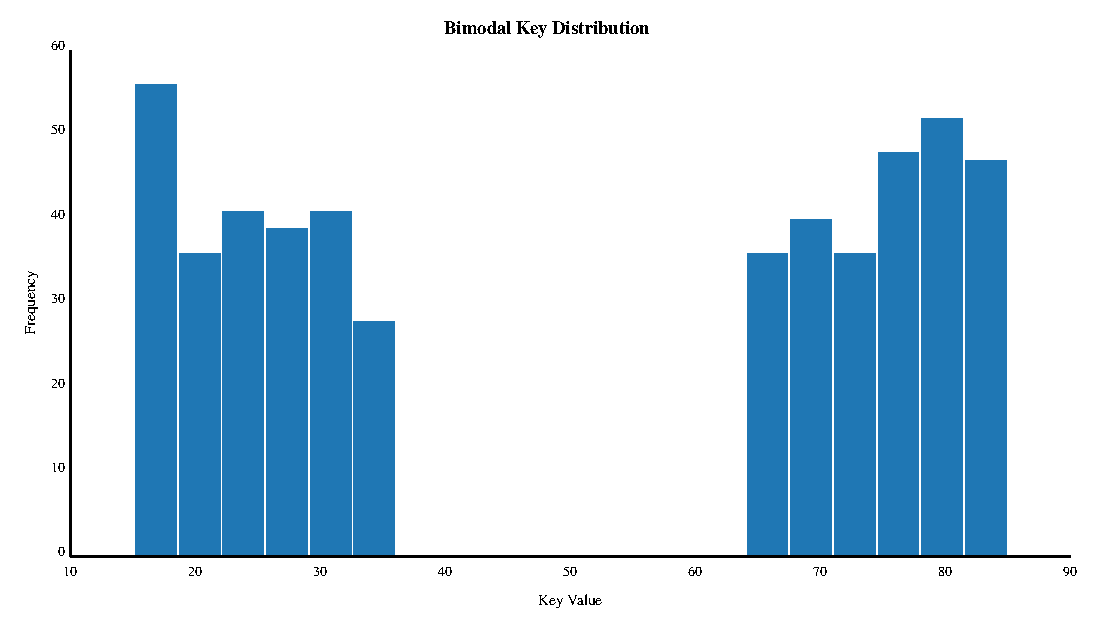
\includegraphics[width=0.85\textwidth]{figures/key_distribution.pdf}
    \caption{A bimodal key distribution. A B-tree treats both clusters identically;
    a learned index allocates more segments to the dense regions and fewer to the
    gaps between them.}
    \label{fig:key-dist}
\end{figure}

However, the sensitivity to distribution is a double-edged sword. Wongkham
et al.\ (PVLDB 2022) showed that while learned indexes outperform traditional
ones on 80\%+ of datasets in single-core settings, they are \textbf{sensitive
to distribution changes} in ways that traditional indexes are not. RMI
prediction error varies from 63 to 1.77 million on OpenStreetMap data, causing
query latencies to range from 440\,ns to 14,212\,ns---a 32$\times$ spread that
B-trees would never exhibit.

%% ====================================================================
\section{The State of the Art (2023--2026)}

The foundational work (2018--2020) established that learned indexes are
viable. The subsequent wave of research has addressed the engineering
challenges---with varying degrees of success.

\subsection{Updatable Learned Indexes}

The static-data assumption of early work has been substantially addressed:

\begin{itemize}[nosep]
    \item \textbf{ALEX} (SIGMOD 2020) introduced gapped arrays with adaptive
        node splitting, analogous to B-tree splits.
    \item \textbf{LIPP} (PVLDB 2021) extended learned trees to eliminate
        prediction deviation on insert, supporting lookup, range query,
        insert, delete, update, and bulk-load.
    \item \textbf{SALI} (SIGMOD 2024) built on LIPP with node-evolving
        strategies for workload-skew adaptation, achieving 2.04$\times$
        insertion throughput over the second-best learned index at 64 threads.
    \item \textbf{Hyper} (SIGMOD 2024) uses two-phase hybrid construction
        (bottom-up leaves, top-down inner nodes), delivering 3.75$\times$
        lookup speedup and 1610$\times$ memory reduction vs.\ prior
        learned indexes.
    \item \textbf{UpLIF} (2025) uses a Balanced Model Adjustment Tree to
        capture updates without full retraining, plus RL-based optimization
        for structure adaptation.
\end{itemize}

Choi et al.\ (SIGMOD 2024) showed that sampled learning can reduce
\textbf{build time} by over 10$\times$ while maintaining accuracy, making
learned indexes construct faster than B-trees---addressing a practical
barrier to adoption.

\subsection{Concurrent Learned Indexes}

Concurrency was largely unaddressed before 2020. It is now an active
sub-area with multiple solutions:

\begin{itemize}[nosep]
    \item \textbf{XIndex} (PPoPP 2020) was the first concurrent learned index,
        using two-phase compaction for writes. 3.2$\times$ over Masstree at
        24 cores.
    \item \textbf{FINEdex} (PVLDB 2022) introduced fine-grained concurrency
        with flattened data arrays and non-blocking retraining. 1.8$\times$
        over XIndex, 2.5$\times$ over Masstree.
    \item \textbf{SALI} (SIGMOD 2024) achieves 2.04$\times$ insertion
        throughput at 64 threads through node-evolving strategies designed
        for concurrent scalability.
    \item \textbf{Hyper} (SIGMOD 2024) delivers up to 5.73$\times$
        improvement in concurrent read-only workloads.
\end{itemize}

However, no concurrent learned index has been shown to \emph{universally}
beat concurrent B-tree variants (OpenBw-Tree, concurrent ART) across
all workloads.

\subsection{LSM-Tree Integration}

The most active sub-area since 2023. LSM-trees dominate write-heavy
workloads (RocksDB, LevelDB, Cassandra), and learned indexes can
accelerate their read path:

\begin{itemize}[nosep]
    \item \textbf{Bourbon} (OSDI 2020) was the first learned index
        integrated with LevelDB's sorted string tables.
    \item \textbf{LearnedKV} (2024) uses a two-tier design: LSM handles
        writes while a learned index accelerates reads. 4.32$\times$ read
        improvement, 1.43$\times$ write improvement over state-of-the-art
        LSM solutions.
    \item \textbf{DobLIX} (PVLDB 2025) is a dual-objective learned index
        for LSM-trees that optimizes both lookup prediction and data access
        from storage, using an RL agent for real-time parameter tuning.
        1.19--2.21$\times$ throughput improvement within RocksDB.
    \item \textbf{Limousine} (SIGMOD 2024) is a self-designing storage
        engine that blends learned and classical indexes across a
        $10^{48}$ design space, auto-generating near-optimal engines for
        given workloads. Up to 3 orders of magnitude better scaling than
        RocksDB, WiredTiger, and FASTER.
\end{itemize}

A comprehensive benchmark (EDBT 2026) evaluated 8 different learned index
designs within LSM-tree systems, identifying a novel configuration space
of design choices specific to LSM integration.

\subsection{String Keys: The Unsolved Problem}

Most learned index research assumes fixed-width integer keys. Variable-length
string keys remain the Achilles' heel:

\begin{itemize}[nosep]
    \item \textbf{LITS} (2024) acknowledges that existing learned indexes
        for strings fail to outperform traditional string indexes (HOT, ART).
        String keys are long, variable-sized, and contain skewed prefixes
        that make last-mile search expensive.
    \item Park et al.\ (PVLDB 2024) proposed memoization-based incremental
        training to avoid full-dataset traversal when retraining string-key models.
    \item \textbf{No learned string index has convincingly beaten ART or HOT}
        in general benchmarks as of 2026.
\end{itemize}

\subsection{GPU Acceleration}

Learned indexes are well-suited to GPUs because model inference is
linear algebra that GPUs accelerate natively:

\begin{itemize}[nosep]
    \item \textbf{G-Learned Index} (IEEE TPDS 2024) enables efficient
        construction and querying on GPU.
    \item \textbf{RTIndeX} (PVLDB 2023) exploits NVIDIA RTX hardware-accelerated
        raytracing cores for database indexing---a creative repurposing of
        GPU hardware.
\end{itemize}

The challenge is that database workloads also need low-latency single-point
lookups where GPU kernel launch overhead dominates.

%% ====================================================================
\section{Production Adoption: The Gap}

Despite hundreds of papers and strong benchmark results, \textbf{no major
database has shipped learned indexes as a core feature} as of early 2026.

\begin{itemize}[nosep]
    \item \textbf{PostgreSQL}: A PGConf.dev 2025 talk explored integrating
        ALEX and CARMI via the access method API. This remains research
        prototyping, not merged into core.
    \item \textbf{RocksDB}: Used as an experimental platform for Bourbon,
        LearnedKV, and DobLIX. No learned index features merged into mainline.
    \item \textbf{Google}: Kraska's original paper came from Google Brain,
        but there is no public confirmation of production deployment in
        Bigtable, Spanner, or other Google systems.
    \item \textbf{MySQL, DuckDB, TiKV}: No known learned index integration.
\end{itemize}

The blockers are not performance---benchmarks consistently show wins for
read-heavy workloads on predictable distributions. The blockers are
\textbf{integration complexity}: buffer managers, query optimizers, WAL,
crash recovery, and the engineering cost of maintaining a second indexing
subsystem alongside battle-tested B-trees.

Andy Pavlo's ``2025 Databases Retrospective'' (CMU, January 2026) discusses
database trends but does not highlight learned indexes as a production
breakthrough.

%% ====================================================================
\section{Existing Implementations}

\subsection{Rust Ecosystem}

\begin{itemize}[nosep]
    \item \textbf{pgm-extra-rs} (2025): High-performance Rust implementation
        of the PGM-Index with \texttt{PgmSet}/\texttt{PgmMap} as drop-in
        replacements for \texttt{BTreeSet}/\texttt{BTreeMap}. Includes a
        dynamic variant supporting inserts and deletes. Benchmarks show
        1.7$\times$ faster queries than \texttt{BTreeSet} on 1M keys and
        3$\times$ less memory. Featured in ``This Week in Rust'' \#628.
    \item \textbf{RMI reference implementation} (MIT/Intel Labs): The official
        Recursive Model Index compiler is written in Rust. It compiles
        learned models into C/C++ source files. Last updated October 2025.
\end{itemize}

\subsection{What Remains Unbuilt}

The \texttt{pgm-extra-rs} crate covers the basic PGM case. What does not
yet exist in Rust (or in production-quality form in any language):

\begin{itemize}[nosep]
    \item \textbf{Concurrent learned indexes}: SALI, Hyper, and FINEdex
        exist as C++ research prototypes. Rust's ownership model is
        well-suited to designing safe concurrent data structures, but
        no Rust implementation exists.
    \item \textbf{LSM-tree integration}: The hottest research sub-area
        has no Rust implementations. Rust-native storage engines
        (e.g., \texttt{sled}) could benefit from learned index integration.
    \item \textbf{String key indexes}: Still unsolved in any language.
        High risk, high potential impact.
\end{itemize}

%% ====================================================================
\section{Conclusion}

Learned indexes replace general-purpose tree traversals with data-aware
mathematical models. The field has matured substantially since Kraska's
2018 paper: updates, concurrency, and LSM integration have moved from
``open problems'' to active sub-areas with competitive solutions.

Yet a gap persists between research benchmarks and production systems. No
major database ships learned indexes. The bottleneck, as PGM++ showed,
may not even be where we expected---memory-bound correction search, not
model quality, often dominates. And string keys remain stubbornly unsolved.

The most promising near-term applications are not in replacing B-trees
wholesale, but in \textbf{hybrid systems}: LSM-trees with learned read
acceleration, self-designing storage engines like Limousine that blend
learned and classical components, and RL-tuned configurations that adapt
to workload shifts. The future of learned indexes is likely not ``learned
indexes vs.\ B-trees'' but ``learned indexes \emph{inside} existing systems,''
quietly improving the read path where the data distribution permits.

\vspace{1em}
\noindent\textbf{Foundational references:}
\begin{itemize}[nosep]
    \item Kraska, T.\ et al.\ ``The Case for Learned Index Structures.''
        \emph{SIGMOD}, 2018.
    \item Ferragina, P.\ and Vinciguerra, G.\ ``The PGM-Index: a fully-dynamic
        compressed learned index with provable worst-case bounds.''
        \emph{PVLDB}, 2020.
    \item Ding, J.\ et al.\ ``ALEX: An Updatable Adaptive Learned Index.''
        \emph{SIGMOD}, 2020.
\end{itemize}

\vspace{0.5em}
\noindent\textbf{Key recent references (2023--2026):}
\begin{itemize}[nosep]
    \item Liu et al.\ ``Why Are Learned Indexes So Effective but Sometimes
        Ineffective?'' (PGM++). \emph{PVLDB} 18(9), 2025.
    \item Hyper: ``High-Performance Learned Index via Hybrid Construction.''
        \emph{SIGMOD}, 2024.
    \item SALI: ``Scalable Adaptive Learned Index.'' \emph{SIGMOD}, 2024.
    \item Limousine: ``Self-Designing Cloud Storage Engines.''
        \emph{SIGMOD}, 2024.
    \item LITune: ``RL-Enhanced Tuning for Learned Indexes.''
        \emph{SIGMOD}, 2025.
    \item DobLIX: ``Dual-Objective Learned Index for LSM-Trees.''
        \emph{PVLDB} 18(11), 2025.
    \item LearnedKV. arXiv:2406.18892, 2024.
    \item ``Evaluating Learned Indexes in LSM-tree Systems.''
        \emph{EDBT}, 2026.
    \item Wongkham et al.\ ``Are Updatable Learned Indexes Ready?''
        \emph{PVLDB} 15(11), 2022.
    \item Choi et al.\ ``Can Learned Indexes be Built Efficiently?''
        \emph{SIGMOD}, 2024.
\end{itemize}

\vspace{2em}
\noindent\small\textit{All figures generated with \texttt{esoc-chart}, a grammar-of-graphics
charting library for Rust.}

\end{document}
